\chapter{Conexões entre neurônios}\label{cap:conexoes}
\section{Introdução}\label{sec:conexoes_intro}
Uma vez visto o comportamento de um neurônio individualmente, este Capítulo traz informações sobre como se dá a conexão entre neurônios. Começando pela conexão direta entre dois neurônios, segue-se com alterações possíveis nessas conexões, além de situações onde é simulada a conexão de diversos neurônios, com comportamentos específicos, implementados com base nos neurônios mostrados anteriormente. Segue, ainda, mostrando um modelo que simula diretamente o comportamento do grupo de neurônios, e finaliza com considerações sobre como o cérebro aprende.

\section{Sinapses}\label{sec:sinapses}
A sinapse é uma conexão entre dois neurônios. Elas podem ser elétricas, que se dão a partir de uma junção entre as duas células, por onde íons podem passar, produzindo uma corrente sináptica proporcional à diferença entre os potenciais de membrana das duas células, ou químicas, que são conectadas através de um espaço entre as células, e a interação entre elas se dá pela liberação de neurotransmissores, que é um elemento químico que se propaga nesse espaço, fazendo a comunicação entre eles. As sinapses químicas são majoritárias no cérebro humano pós-natal, enquanto que as elétricas estão presentes em quantidade relevante apenas durante o período de desenvolvimento embrionário humano. As sinapses químicas são categorizadas em excitatórias ou inibitórias, de acordo com o efeito no potencial de membrana da célula pós-sináptica (a que responde à liberação do neurotransmissor após o potencial de ação do neurônio pré-sináptico). Enquanto as sinapses excitatórias despolarizam a membrana, as inibitórias causam hiperpolarização, facilitando ou dificultando, respectivamente, o potencial de ação da célula pós-sináptica. Os neurotransmissores mais comuns associados aos neurônios corticais são o \textbf{glutamato}, que excita a célula pós-sináptica, e o \textbf{ácido $\gamma$-aminobutírico (GABA)}, que, normalmente, a inibe\footnote{No cérebro pré-natal o GABA é excitatório \cite{ben-ari_excitatory_2002}}.
O esquema de uma sinapse química é mostrado na Figura~\ref{fig:sinapses}. Os neurotransmissores são transportados por compartimentos ao redor da membrana neuronal chamados de vesículas.
\begin{figure}[tb]
	\centering
	\caption{Esquema simplificado de uma sinapse química}
	\label{fig:sinapses}
	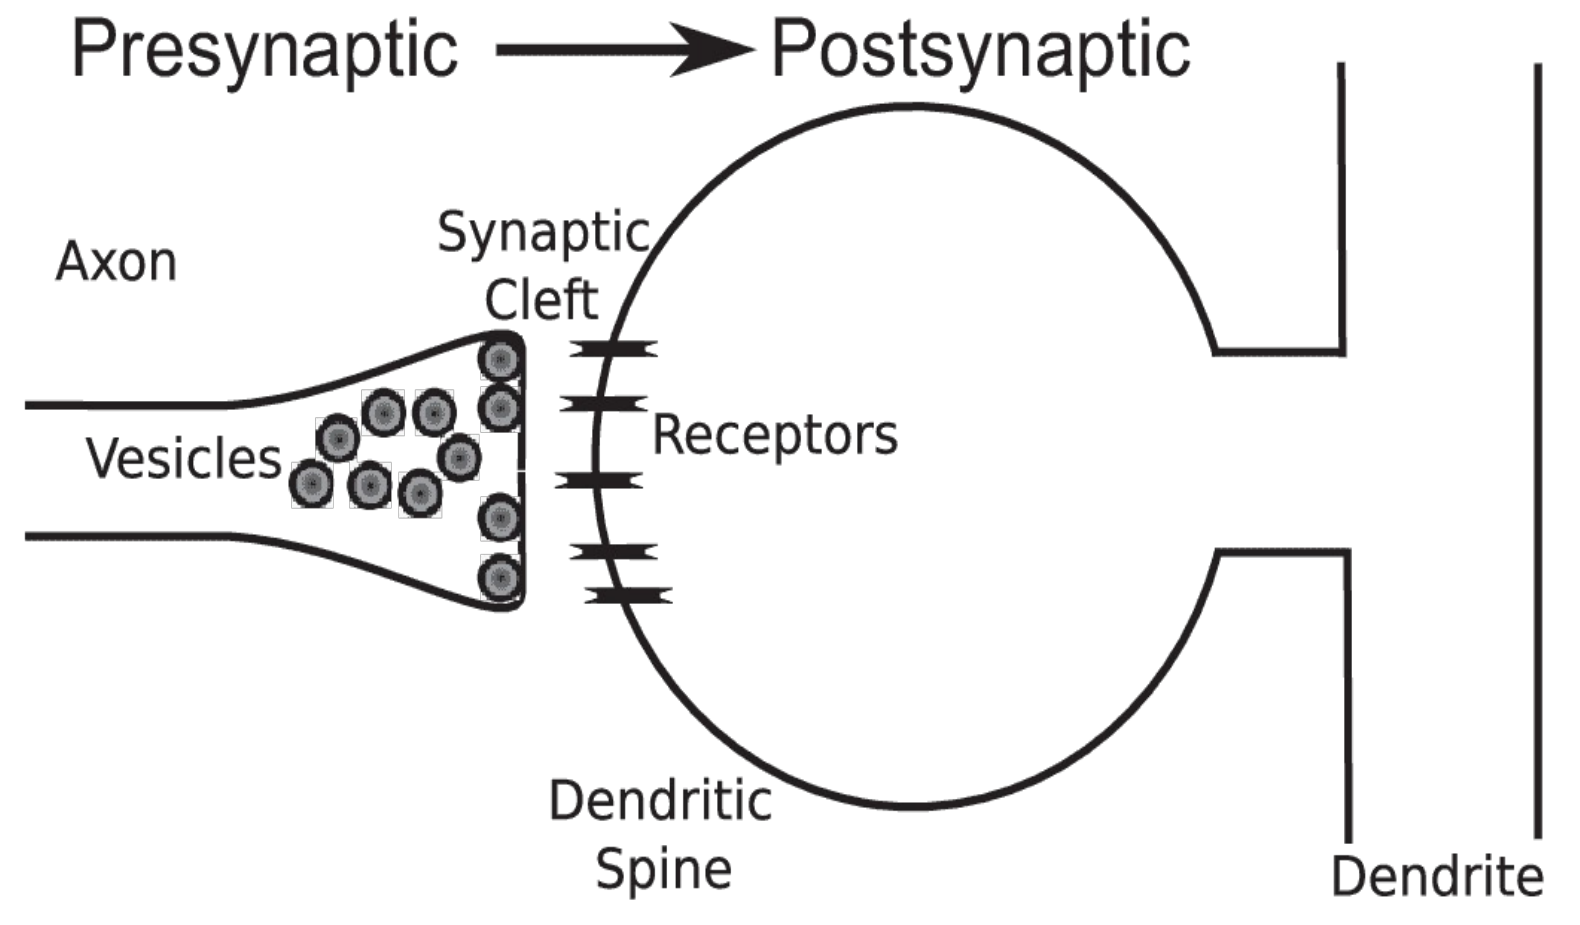
\includegraphics[width=0.7\linewidth]{figs/sinapses}\\
	\small{Fonte: \cite{miller_introductory_2018}}
	%TODO: trocar figura
\end{figure}

A transmissão sináptica é modelada usando a equação abaixo \cite{dayan_theoretical_2001}:
\begin{equation}\label{eq:sinapse}
	\frac{dG_{sin}(t)}{dt}=\frac{-G_{sin}(t)}{\tau_{sin}}
\end{equation}
sendo $G_{sin}(t)$ a condutância sináptica e $\tau_{sin}$ a constante de tempo específica para o tipo de sinapse. Além disso, se houver disparo da célula pré-sináptica, ocorre o seguinte mapeamento:
\begin{equation}\label{eq:sinapse_mapeamento}
	G_{sin}(t)\mapsto G_{sin}(t)+\Delta G
\end{equation}
onde $\Delta G$ é o incremento de condutância. Um modelo mais elaborado considera o crescimento e decaimento de condutância usando a equação abaixo \cite{miller_introductory_2018}:
\begin{equation}\label{eq:sinapse_delta}
	\Delta G_{sin}(t)=\frac{\Delta G}{K}e^{-(t-t_{disparo})/\tau_{decai}}\Big[1-e^{-(t-t_{disparo})/\tau_{cresce}}\Big]
\end{equation}
com $\tau_{cresce}$ a constante de crescimento, $\tau_{decai}$ a de decaimento ($\tau_{decai}>\tau_{cresce}$), $t_{disparo}$ o instante do disparo da célula pré-sináptica, e $K$ um fator para garantir que a condutância tenha um valor máximo igual a $\Delta G$, calculado por:
\begin{equation}\label{eq:sinapse_k}
	K=\Bigg(\frac{\tau_{decai}}{\tau_{cresce}+\tau_{decai}}\Bigg)\Bigg(\frac{\tau_{cresce}}{\tau_{cresce}+\tau_{decai}}\Bigg)^{\tau_{cresce}/\tau_{decai}}
\end{equation}
A dinâmica da condutância sináptica é mostrada na Figura~\ref{fig:respostasinaptica}, onde é possível observar o incremento da condutância sináptica (curva de cima) após a ocorrência de um potencial de ação (linhas verticais do gráfico embaixo).

\begin{figure}[tb]
	\centering
	\caption{Condutância sináptica em resposta aos potenciais de ação da célula pré-sináptica}
	\label{fig:respostasinaptica}
	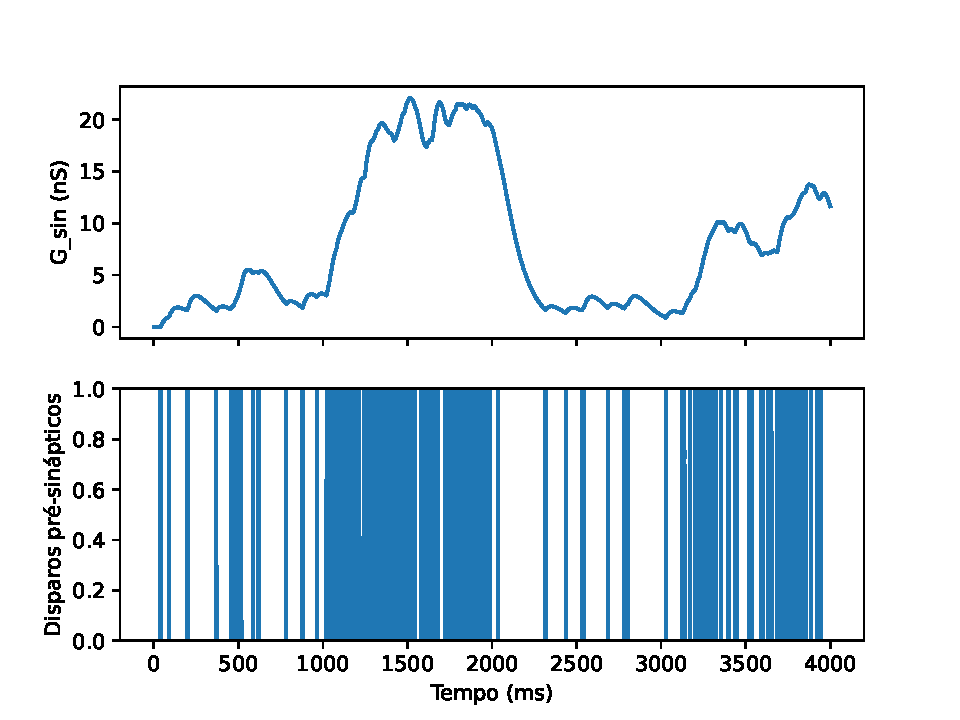
\includegraphics[width=0.7\linewidth]{figs/resposta_sinaptica}
	%TODO: regerar
\end{figure}

\subsection{Sinapses dinâmicas}\label{subsec:sinapses_dinamicas}
Acima, os modelos de sinapses possuem pesos fixos. Entretanto, fisiologicamente, as condutâncias sinápticas não são fixas, mas mudam de acordo com a disponibilidade de recursos sinápticos no terminal pré-sináptico, determinados por algumas condições de entrada. Esse comportamento é chamado de sinapse dinâmica, cuja força da conexão varia em um curto período de tempo, ocasionando o a chamada plasticidade de curto prazo (PCP), ou de curta duração. Experimentalmente, são observados dois tipos, com efeitos opostos na eficácia sináptica, como mostrados na Figura~\ref{fig:plasticidadecurtaduracao}. À esquerda, é exibido o fenômeno da depressão de curta duração, que causa uma redução temporária na força sináptica, e à direita o fenômeno da facilitação de curta duração, que causa um incremento temporário.
\begin{figure}[tb]
	\centering
	\caption[Depressão e facilitação sináptica]{Depressão e facilitação sináptica}
	\label{fig:plasticidadecurtaduracao}
	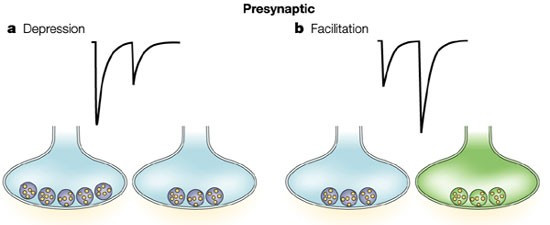
\includegraphics[width=0.7\linewidth]{figs/plasticidade_curta_duracao}
	%TODO: trocar figura
\end{figure}
O modelo matemático da PCP é fundamentado no conceito de uma quantidade limitada de recursos sinápticos disponíveis para transmissão, tal como a quantidade total de vesículas sinápticas. Esse número de recursos pré-sinápticos muda dinamicamente de acordo com o histórico recente de picos de atividade. Após um pico pré-sináptico, a probabilidade de liberação do conjunto disponível para utilização aumenta devido ao influxo de cálcio induzido pelo pico no terminal pré-sináptico. A simulação de depressão e facilitação sinápticas pode ser feita alterando-se o valor de $\Delta G$ acima para:
\begin{equation}\label{eq:sinapse_facilitacao_depressao}
	\Delta G=G_{max}p_0FD
\end{equation}
com $G_{max}$ o valor máximo de condutância sináptica, $p_0$ a probabilidade de liberação do neurotransmissor, e $F$ e $D$ as variáveis de facilitação e depressão sináptica, atualizadas por:
\begin{equation}\label{eq:depressao_sinaptica}
	\frac{dD}{dt}=\frac{1-D}{\tau_D}
\end{equation}
\begin{equation}\label{eq:facilitacao_sinaptica}
	\frac{dF}{dt}=\frac{1-F}{\tau_F}
\end{equation}
e, seguindo cada disparo da célula pré-sináptica, ocorrem os seguintes mapeamentos:
\begin{equation}\label{eq:mapeamento_depressao_sinaptica}
	D\mapsto D-p_0FD
\end{equation}
\begin{equation}\label{eq:mapeamento_facilitacao_sinaptica}
	F\mapsto F+f_{fat}(F_{max}-F)
\end{equation}
com $F_{fat}$ denotando o grau de facilitação ($0\leq f_{fat}\leq 1$) e $F_{max}$ o seu valor máximo.

\section{Multi-estabilidade}\label{sec:biestabilidade}

\subsection{Oscilações e multi-estabilidade}
Além das alterações de comportamento causadas pelas entradas aplicadas (injeção de corrente), os neurônios podem mudar sua resposta de acordo com as conexões feitas uns com os outros. A capacidade dos neurônios de manter múltiplos estados de atividades mesmo recebendo valores idênticos de entrada é chamada de \textbf{multi-estabilidade}. O próprio neurônio de Hodgkin-Huxley, visto anterior, podes alternar entre um estado de quiescência, exibindo oscilações sub-limiares (variações no potencial de membrana insuficientes para a produção de um potencial de ação), e um estado de ressonância, que é uma resposta recorrente, conforme mostrado na Figura~\ref{fig:hhdinamico}. Nos três cenários é aplicado um pulso de corrente no intervalo de $0,05$ até $0,45\ s$, porém variando a amplitude. É possível observar que, para $0,300\ nA$ (no topo) ocorre apenas um disparo de potencial de ação, com uma oscilação em seguida. Para $0,624\ nA$ (no meio), alguns disparos acontecem, porém não o suficiente para ativar o comportamento ressonante, que é conseguido com um leve incremento de corrente, para $0,626\ nA$ (embaixo).

\begin{figure}[tb]
	\centering
	\caption{Comportamento variado do modelo de Hodgkin-Huxley para diferentes correntes}
	\label{fig:hhdinamico}
	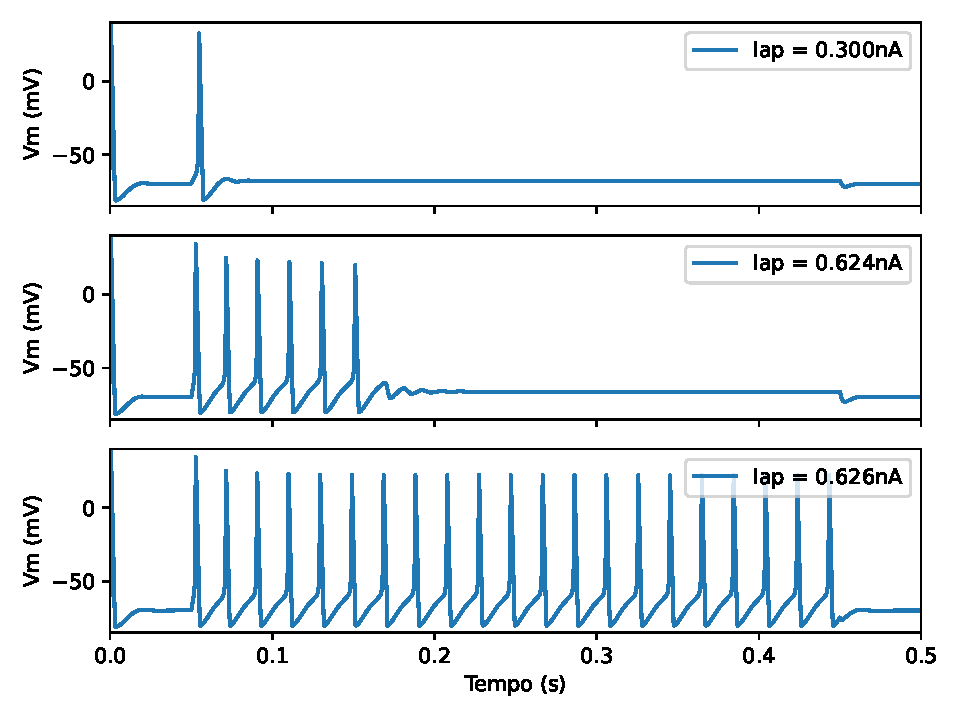
\includegraphics[width=0.7\linewidth]{figs/hh_dinamico}
	%TODO: regerar
\end{figure}
A forma mais simples de multi-estabilidade é a bi-estabilidade, onde, com um mesmo estímulo, dois estados de atividade neuronal podem ocorrer, gerando a chamada rivalidade perceptual, onde estímulos únicos podem ser percebidos de mais de uma maneira, alterando entre cada um dos perceptos (percepções bi-estáveis), como no exemplo da Figura~\ref{fig:cubonecker}, uma ilusão de ótica onde o cubo, conhecido como Cubo de Necker, pode ser visto com a face frontal em lugares diferentes.
% Já na Figura~\ref{fig:cao_homem}, ora a imagem aparenta ser um cachorro visto de frente, ora parece um homem de costas.

\begin{figure}[tb]
	\centering
	\caption[Cubo de Necker]{Cubo de Necker}
	\label{fig:cubonecker}
	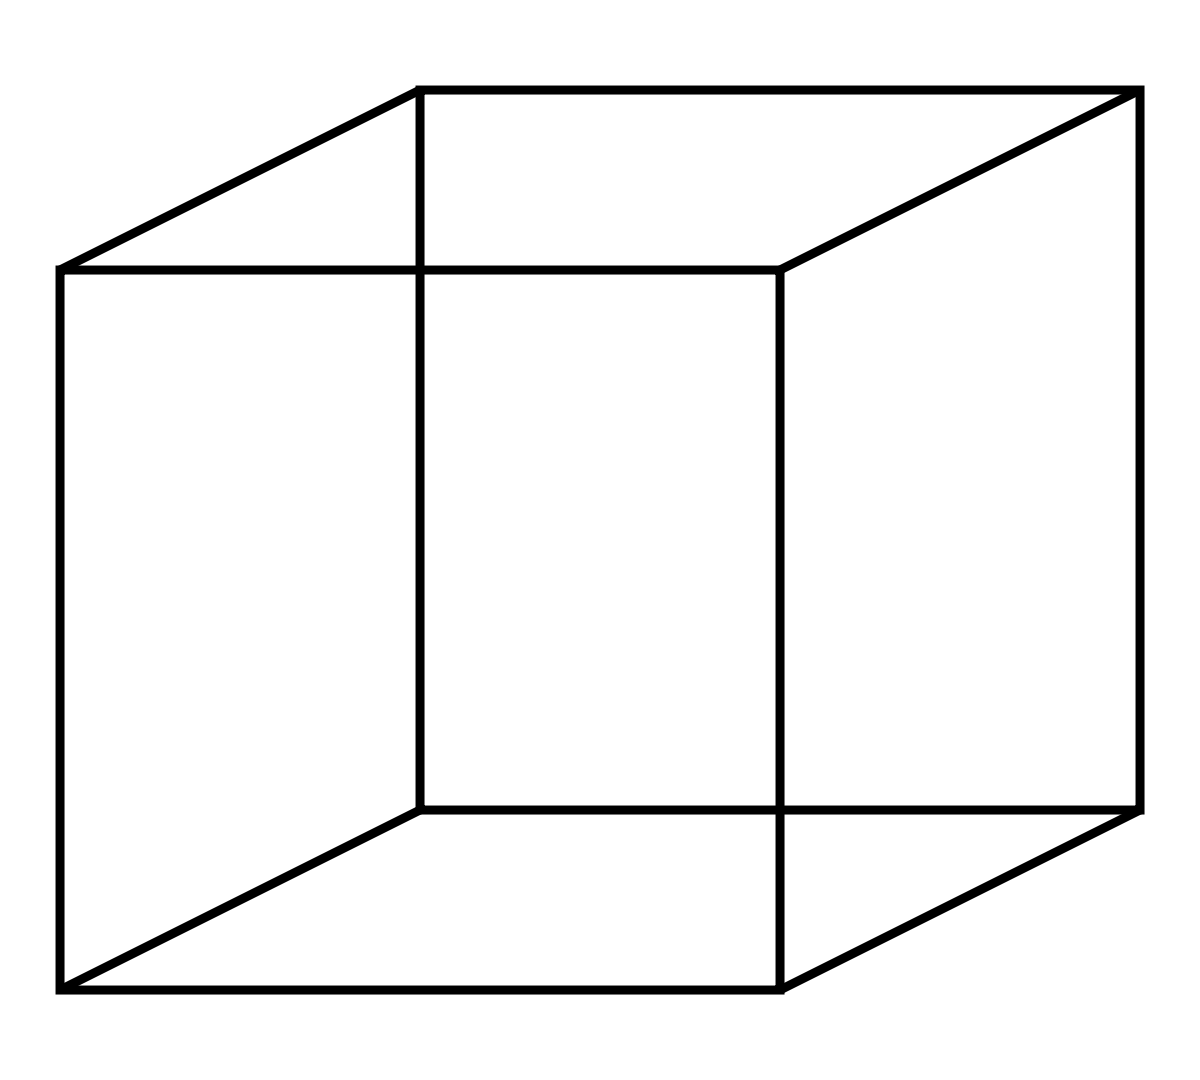
\includegraphics[width=0.7\textwidth]{figs/cubo_necker}
	\fonte{Domínio público}
\end{figure}

Quando são simuladas as conexões entre um grupo de neurônios, é conveniente considerar a atividade média deles, ou seja, a taxa de disparo dentre eles, e esse conjunto de neurônios é chamado de \textbf{unidade}. No caso da bi-estabilidade, por exemplo, duas unidades rivalizam entre si, conforme mostrado na Figura~\ref{fig:unidadesdecisao}. No exemplo, $s_1$ e $s_2$ são os estímulos, diferenciados apenas pela eventual presença de ruído. As saídas $r_1$ e $r_2$ são as taxas médias de disparo de cada unidade, e cada uma delas também serve como entrada para a mesma, comportamento chamado de \textbf{\textit{feedback} recorrente}. Além disso, há uma interconexão entre as unidades, com a saída de uma se tornando entrada de outra. Tanto as entradas quando as conexões recorrentes são excitatórias (representadas pelos triângulos no topo das unidades), reforçando a taxa de disparo, enquanto as interconexões são inibitórias (representadas pelos círculos pretos). $W^{EE}$ e $W^{IE}$ são as forças das conexões, com o $EE$ indicando a conexão excitatória e $IE$ a inibitória, e $s^E$ e $s^I$ são a fração de canais sinápticos excitatórios e inibitórios, respectivamente, que estão abertos, e são função da taxa de disparos. Além do ruído na entrada, pode ocorrer ruído dentro das unidades, e a presença de ambos pode induzir às transições entre estados bi-estáveis.


\begin{figure}[tb]
	\centering
	\caption[Unidades de decisão com feedback recorrente e interconexão]{Unidades de decisão com feedback recorrente e interconexão}
	\label{fig:unidadesdecisao}
	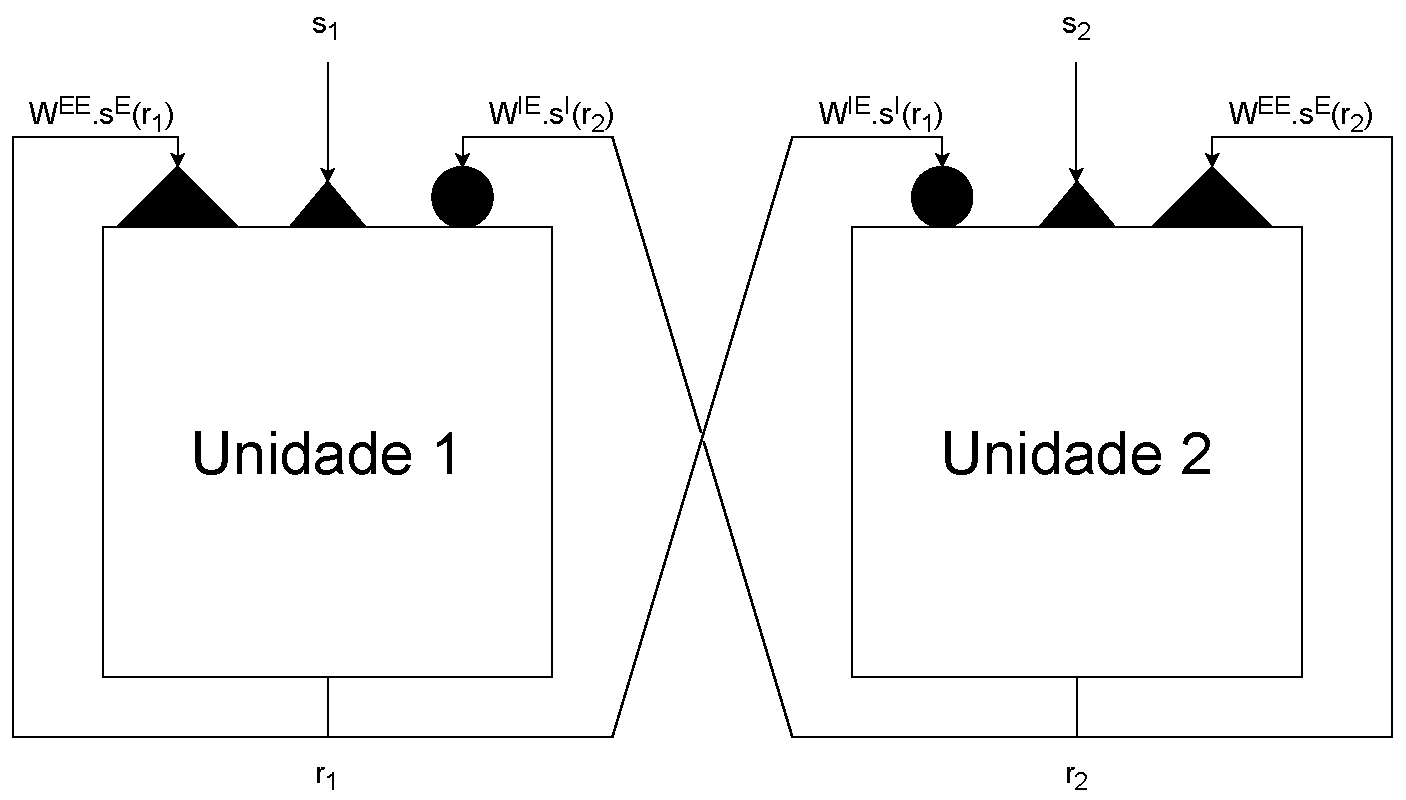
\includegraphics[width=0.7\linewidth]{figs/unidades_decisao}
	\fonte{O autor (\the\year)}
\end{figure}

\subsection{Circuitos de multi-estabilidade}
Um circuito conhecido de multi-estabilidade é o \textbf{gerador de padrão central} (\textit{central pattern generator}, CPG, em inglês), que são circuitos neurais que podem reproduzir padrões rítmicos de atividade neuronal sem receber entradas rítmicas~\cite{ijspeert_central_2008}. Eles são fundamentais, dentre outras coisas, para circuitos neurais associados à locomoção.

\begin{figure}[tb]
	\centering
	\caption[Gerador de padrão central de duas unidades]{Gerador de padrão central de duas unidades}
	\label{fig:cpg}
	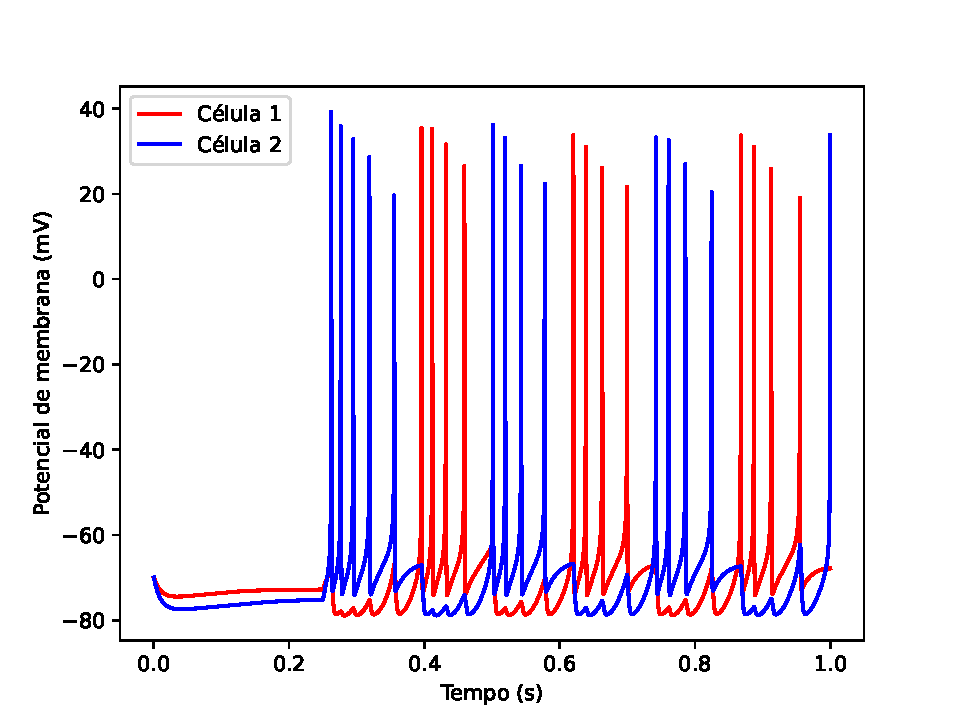
\includegraphics[width=0.7\linewidth]{figs/cpg}
	\fonte{O autor (\the\year)}
\end{figure}
Um exemplo do seu comportamento é exibido na Figura~\ref{fig:cpg}. Nela, são exibidas as curvas do potencial de membrana de membrana de duas unidades, conectadas como mostrado anteriormente, e com um pulso de corrente aplicado por volta de $0,25\ s$. É possível observar que, quando a célula 1 é ativada (representado pelo disparo dos potenciais de ação), a célula 2 é inibida. O contrário também ocorre, com a célula 1 sendo inibida com a ativação da célula 2, alternando entre qual das unidades dispara durante um intervalo de tempo. Não há o disparo simultâneo das duas células. Um correlato dessa atividade com a locomoção é o movimento das duas pernas humanas. Se associarmos cada perna com uma unidade, hora uma delas está em movimento (uma célula ativada), hora é a outra, alternando ao longo do tempo. Circuitos geradores de padrão central são bastante empregados no projeto de locomoção de robôs articulados~\cite{ijspeert_central_2008}.

Outros circuitos conhecidos de multi-estabilidade são os de tomada de decisão. Esses circuitos acumulam informações sensoriais ao longo do tempo até que uma decisão possa ser tomada. A computação da informação pode ser feita simplesmente integrando a atividade neural ao longo do tempo~\cite{cain_computational_2012}, como pode ser visto na Figura~\ref{fig:tomadadecisao}. Neste exemplo, um estímulo é aplicado simultaneamente (instante $0\ s$) em duas unidades, também conectadas como acima, que acumulam as evidências desse estímulo ao longo do tempo, alterando a taxa de disparo média das unidades. Neste caso, a decisão tomada, ou seja, a unidade escolhida, é a que atingir primeiro um determinado limiar, definido como a taxa de disparo de $40\ Hz$. A unidade 1 (em azul) foi a vencedora.
\begin{figure}[tb]
	\centering
	\caption[Circuito de tomada de decisão]{Circuito de tomada de decisão}
	\label{fig:tomadadecisao}
	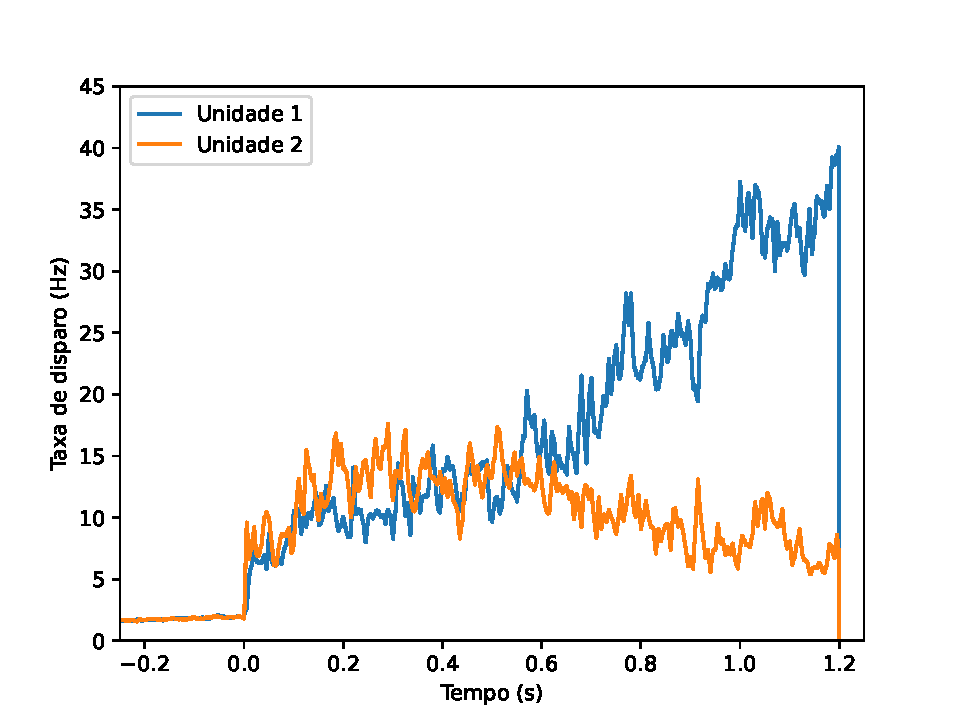
\includegraphics[width=0.7\linewidth]{figs/tomada_decisao}
	\fonte{O autor (\the\year)}
\end{figure}

\section{Modelos de taxa de disparo}\label{sec:modelostaxa}
Nos exemplos acima, os cálculos de taxa de disparo são feitos simulando vários neurônios individualmente. Mesmo usando modelos mais simplificados, como os de integra-e-dispara, esse estratégia pode não ser muito adequada, principalmente do ponto de vista da eficiência computacional, onde a simulação de um grande número de neurônios (milhares ou dezenas de milhares) pode se tornar impraticável mesmo utilizando computadores mais robustos. Nesses casos, convém utilizar um modelo que fornece a taxa de disparo. Sem dúvidas, o mais conhecido deles é o de Wilson-Cowan~\cite{wilson_excitatory_1972}. Esse modelo leva em consideração as subpopulações (unidades) de neurônios excitatórios e inibitórios separadamente, levando em conta o chamado \textbf{Princípio de Dale}, onde cada neurônio é classificado como puramente excitatório ou inibitório, não podendo ser os dois ao mesmo tempo~\cite{dale_pharmacology_1935}.

As equações do modelo de Wilson-Cowan possuem o formato abaixo, com a Equação~\ref{eq:wilson_cowan_e} referente à variação da taxa de disparos para a população de neurônios excitatórios, e a Equação~\ref{eq:wilson_cowan_i} para a população de neurônios inibitórios:
\begin{align}
	\tau_e\frac{\mathrm{d}r_e}{\mathrm{d}t} &=-r_e+F_e(w_{ee}r_e-w_{ie}r_i+T_e(t))\label{eq:wilson_cowan_e}\\
	\tau_i\frac{\mathrm{d}r_i}{\mathrm{d}t} &=-r_i+F_i(w_{ei}r_e-w_{ii}r_i+T_i(t))\label{eq:wilson_cowan_i}
\end{align}
sendo $T_e(t)$ e $T_i(t)$ as entradas do modelo, $r_e$ e $r_i$ as taxas de disparo, $\tau_e$ e $\tau_i$ as constantes de tempo, $w_{ee}$ e $w_{ii}$ os pesos das conexões excitatórias (recorrentes) e $w_{ie}$ e $w_{ei}$ os pesos das conexões inibitórias. $F$ é uma função de ativação que nesse caso, define a fração de neurônios que disparam para cada subpopulação.

O comportamento observado ao simular o modelo de Wilson-Cowan é exibido na Figura~\ref{fig:wilson_cowan}. A atividade, em termos de taxa de disparo de cada subpopulação, pode convergir para um valor estável em regime permanente, como mostrado na Figura~\ref{fig:ww_atividade}. Após aproximadamente $50\ ms$, as taxas de disparo não se alteram, para ambas as subpopulações. Esse modelo também possui uma significância importante em comparação à outros trabalhos por ser uma introdução formal de ferramentas para análise de sistemas dinâmicos em neurociência~\cite{ramezanian-panahi_generative_2022}. De maneira simplificada, sistemas dinâmicos são aqueles onde as variáveis mudam ao longo do tempo, como no caso das taxas de disparo se alterando. Quando as taxas de disparo de cada população não se alteram, a curva que representa a trajetória delas é chamada de \textbf{\textit{nullcline}} (isóclina de inclinação nula, em tradução livre), ocorrendo quando as derivadas das equações \ref{eq:wilson_cowan_e} e \ref{eq:wilson_cowan_i} são iguais a zero, como mostradas na Figura~\ref{fig:ww_trajetoria}, sendo a curva em vermelho para a subpopulação excitatória, e em verde para a inibitória. A curva em azul representa a trajetória do sistema como um todo, que converge para o ponto de interseção entre as curvas das duas subpopulações, onde ambas as taxas não se alteram, sendo este o ponto de equilíbrio do sistema. As setas na cor cinza representam as trajetórias das alterações do sistema em direção ao ponto de equilíbrio.
\begin{figure}
	\centering
	\caption{Comportamento das simulações do modelo de Wilson-Cowan}
	\label{fig:wilson_cowan}
	\begin{subfigure}[b]{0.49\textwidth}
		\caption{Atividade}
		\label{fig:ww_atividade}
		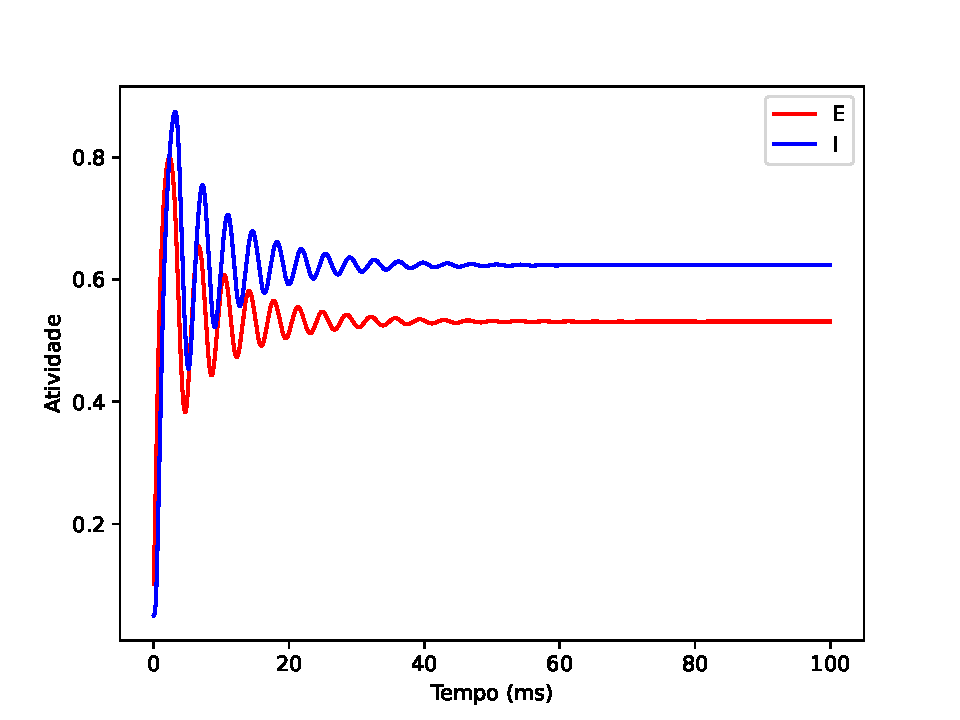
\includegraphics[width=\textwidth]{figs/ww_atividade}
	\end{subfigure}
	~
	\begin{subfigure}[b]{0.49\textwidth}
		\caption{Trajetória}
		\label{fig:ww_trajetoria}
		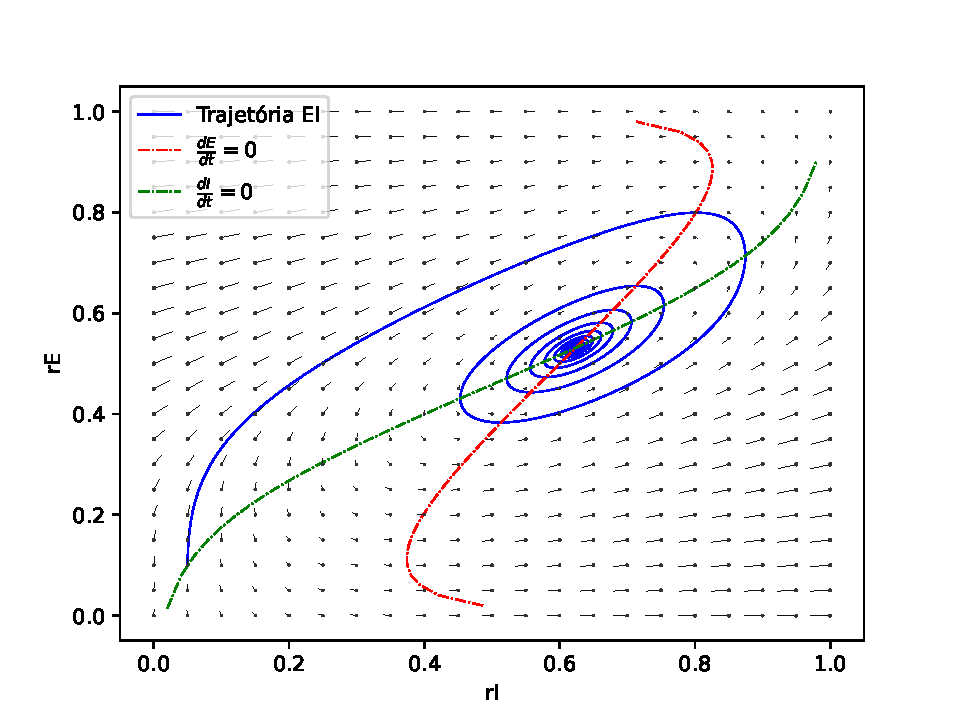
\includegraphics[width=\textwidth]{figs/ww_trajetoria}
	\end{subfigure}
	\legend{Fonte: o autor (\the\year)}
\end{figure}

\section{Aprendizado e plasticidade de longa duração}\label{sec:aprendizado}

A plasticidade é a capacidade do cérebro de se adaptar, tanto estrutural quanto funcionalmente, em resposta à estímulos externos~\cite{mateos-aparicio_impact_2019}. O termo se torno bastante conhecido principalmente devido à chamada \textbf{Regra de Hebb}, que diz que se um neurônio A excita um neurônio B repetidas vezes, contribuindo para o disparo deste, então a sinapse entre os dois deve ser fortalecida~\cite{hebb_organization_2005}. Diferentemente das alterações de curta duração mostradas na Seção~\ref{subsec:sinapses_dinamicas}, as mudanças das forças de conexões neuronais da plasticidade sináptica persistem por longos períodos de tempo. Um exemplo é o conceito de \textbf{potencialização de longa duração} (\textit{long-term potentiation, LTP, em inglês}), que se trata de um crescimento da força de conexão sináptica que duram por algumas dezenas de minutos~\cite{bliss_longlasting_1973}. Do mesmo modo, há a \textbf{depressão de longa duração} (\textit{long-term depression, LTD, em inglês}), que é a diminuição da força de conexão por um longo período de tempo~\cite{bear_long-term_1996}. A regra de plasticidade mais simples é dada pela equação abaixo:
\begin{equation}\label{eq:regra_hebb}
	\tau_w\dfrac{\mathrm{d}\mathbf{w}}{\mathrm{d}t}=v\mathbf{u}
\end{equation}
onde $\tau_w$ é uma constante de tempo que controla a taxa em que os pesos se atualizam, $\mathbf{w}$ é o vetor de pesos sinápticos, $v$ é a atividade do neurônio pós-sináptico e $\mathbf{u}$ o vetor de atividades dos neurônios pré-sinápticos.

Na versão simplificada de plasticidade exibida acima, tanto a atividade do neurônio pré-sináptico quanto a do pós aumentam a força da conexão. Na prática, porém, há uma espécie de competição entre diferentes sinapses, que pode ser observada na chamada \textbf{plasticidade dependente do tempo de disparo} (\textit{spike-timing dependent plasticity}, STDP, em inglês), que depende do tempo relativo do disparo das células pré e pós-sinápticas, como exibido na Figura~\ref{fig:stdp}~\cite{song_competitive_2000}.
\begin{figure}[tb]
	\centering
	\caption[Plasticidade dependente do tempo de disparo (STDP)]{Plasticidade dependente do tempo de disparo (STDP)}
	\label{fig:stdp}
	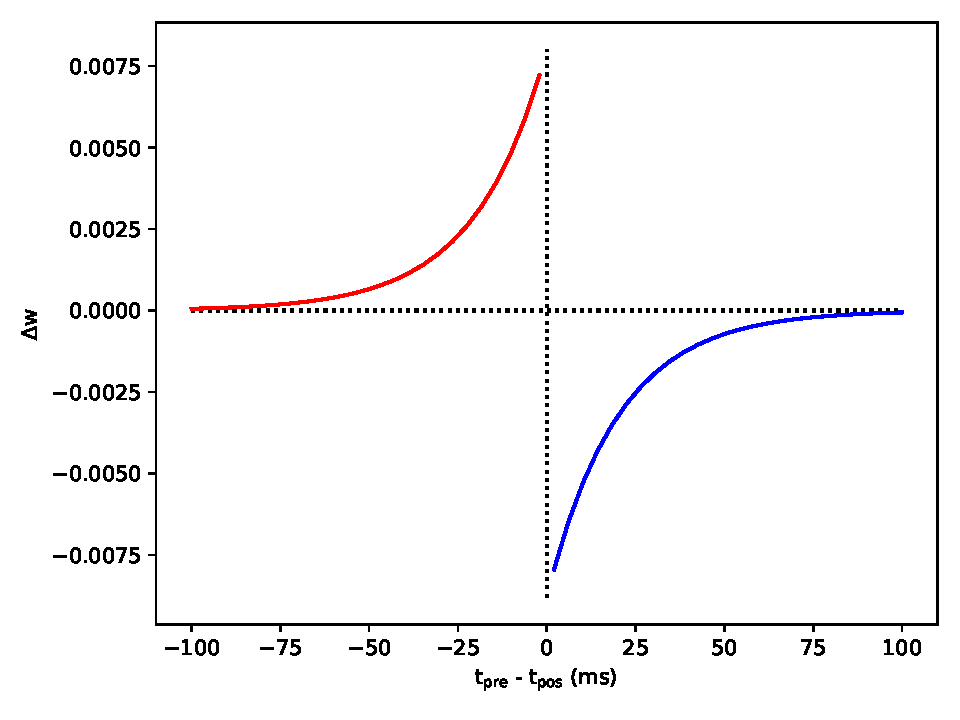
\includegraphics[width=0.7\linewidth]{figs/stdp}
	\legend{Fonte: o autor (\the\year)}
\end{figure}
Na abscissa é apresentada a diferença de tempo entre os disparos dos neurônios pré e pós-sinápticos. 0~(zero) significa que ambos disparam ao mesmo tempo, valores negativos estão associados ao neurônio pré-sináptico disparando primeiro, e valores positivos ao disparo do neurônio pós-sináptico primeiro. Na primeira situação, com o pré seguido do pós (curva em vermelho), a atividade resulta em uma potencialização de longa duração, com a diferença de peso sendo maior proporcionalmente à diminuição do tempo entre os disparos, até próximo de 0~(zero), enquanto na situação onde o pós-sináptico dispara primeiro (curva em azul), a atividade resulta em uma depressão de longa duração, também com a diferença de peso aumentando proporcionalmente com a diminuição da diferença de tempo entre os disparos.

A modelagem da STDP é dada pela equação abaixo~\cite{song_competitive_2000}:
\begin{equation}\label{eq:stdp}
	\Delta_w=\begin{cases}
		A_+\exp(\Delta t/\tau_+)\quad\text{se }\Delta t<0\\
		-A_-\exp(-\Delta t/\tau_-)\quad\text{se }\Delta t\geq0
	\end{cases}
\end{equation}
sendo $A_+$ e $A_-$ os valores máximos de modificação sináptica, ambos com valor positivo e o máximo próximo de $\Delta_t=0$. $\tau_+$ e $\tau_-$ são as faixas de intervalo entre disparo das células pré para pós-sinápticas. A STDP é uma das bases de aprendizado de diversos algoritmos de aprendizado de máquina, que serão apresentados no Capítulo seguinte.
